\documentclass[11pt,a4paper,margin=1.5in]{article}
\usepackage{amsfonts}
\usepackage{amssymb}
\usepackage{amsmath}
\usepackage{color}
\usepackage{setspace}
\usepackage{dcolumn}
\newcolumntype{d}[1]{D{.}{.}{#1}}
\usepackage{multicol}

\usepackage[dvipsnames]{xcolor}
\definecolor{cobalt}{rgb}{0.0, 0.28, 0.67}
\definecolor{darkblue}{rgb}{0.0, 0.0, 0.55}
\definecolor{darkpowderblue}{rgb}{0.0, 0.2, 0.6}
\definecolor{egyptianblue}{rgb}{0.06, 0.2, 0.65}
\usepackage[pdfencoding=auto]{hyperref}
\hypersetup{
    colorlinks=true,
    linkcolor=black,%egyptianblue,
    citecolor=black,%blue,
    filecolor=magenta,      
    urlcolor=darkblue,
}
\hypersetup{pdfstartview={XYZ null null 0.80}}

\usepackage[FIGTOPCAP]{subfigure}
\usepackage{IEEEtrantools}
\usepackage{extsizes}
\usepackage{tikz}
\usepackage{pgfplots}
%\usepackage{subcaption}
\usepackage{booktabs}
\usepackage[flushleft]{ threeparttable}
\usepackage{graphicx}
\usepackage{epstopdf}
\usepackage{parskip}
\usepackage{geometry}
\usepackage{pdflscape}
\usepackage{rotating}
%\usepackage{afterpage}
\usepackage{multirow}
\usepackage{natbib}
\usepackage{xfrac}
\usepackage{paralist}
\usepackage{fancyhdr}
%\usepackage[nomarkers, nolists]{endfloat}
%\renewcommand{\efloatseparator}{\vspace{3in}}

%\theoremstyle{plain}
\newtheorem{assumption}{Assumption}

\setlength{\parindent}{12pt}
%\onehalfspacing
\doublespacing

\defcitealias{IMF:2013}{IMF, 2013}
\defcitealias{Blanchard:2016}{Blanchard, 2016}

\title{A Fisher Ideal Take on Fiscal Debt}
%\thanks{
%	I'd like to thank Bill Barnett, David Beckworth, Markus Brunnermeier, Josh Hendrickson, Tom Holden, John Nana Francois, Peter Ireland, Eric Leeper, Ryan Mattson, and Ricardo Nunes for their helpful comments and advice on this and previous versions of this paper.
%	I'd also like to thank the numerous seminar participants at the University of Kansas, Utah State University, Southern Utah University, and various conferences for their invaluable feedback.}}
\author{Andrew Keinsley\thanks{Associate Professor of Economics, Weber State University --- Email: andrewkeinsley@weber.edu -- Address: Department of Economics WB 226, 1337 Edvalson St, Ogden, UT 84408-3807 } \\  {\small Weber State University}}
%\date{ {\bf Preliminary: Comments Welcome}  \\ This Version: \today}

\begin{document}
\maketitle
\thispagestyle{empty}

\begin{abstract}
\noindent This paper derives a Fisher ideal quantity index of US Treasury debt.

%monetary services channel to the fiscal theory of the price level.
\end{abstract}
\vspace{2em}

\noindent{Keywords}: Fisher Ideal Index, Aggregation Theory, Fiscal Debt
\newpage
\setcounter{page}{1}


\section{Introduction}

% Introduce the Topic and its Imporance
The fiscal response to the COVID crisis in the US and the ensuing rise of inflation and interest rates has brought the concept of ``fiscal capacity" back into the spotlight. 
Despite growing debt levels, borrowing costs trended downward from the 1980s until the US financial crisis in the late 2000s.
%Forecasters, despite accelerating debt levels, suggest that short-term interest rates will peak somewhere around two percent in the post-COVID cycle. 
All of this suggests that there must be more to the fiscal-capacity discussion than just the stock of outstanding principal values.
If that additional component could be discovered, could it also shed light on the connection between debt and the macroeconomy, like the fiscal theory of the price level (FTPL)?

% Brief Literature Review
\citet{Krishnamurthy-VissingJorgensen:2012}, \citet{Krishnamurthy-VissingJorgensen:2013}, and \citet{Nagel:2016}---to name just a few---have established that the value of fiscal debt in the US is much more than the sum of its outstanding stock of principal. 
\citet*{Caballero-Farhi-Gourinchas:2017} build on this idea to explain historically low borrowing costs in the face of historically high debt levels.
More recently, \citet*{Brunnermeier-Merkel-Sannikov:2022} applied these concepts to the fiscal capacity and the FTPL literatures. 
They show that the demand side of this debt market raises the borrowing limits of the fiscal authority because the additional debt provides safety or transaction services, which I'll refer to more generally as monetary services.\footnote{
	These monetary services generally include the aforementioned transactions services as well as other attributes such as liquidity, safety, use as collateral, etc.}
Theoretically, they show that the inclusion of these monetary services disrupt the traditional FTPL channel \citep[see][as a seminal example]{Leeper:1991} and, along with the empirical results of \citet{Jiang-etal:2019}, suggest that this channel is important in the valuation of Treasury debt. 
%, but introduce the possibility of other channels.\footnote{
%	\citet{Cui-Soren:2019} find that the bubble term in their model with low interest rates is primarily composed of liquidity services as well.}
This paper explores this monetary service channel in more depth, aiding in our understanding of debt dynamics and their impact on the economy as a whole. 

% Purpose of this paper...
The purpose and contribution of this paper is two-fold.
%to measure the monetary services of marketable fiscal debt in the US and to estimate their impact on inflation.
% Contribution to the literature
%The contribution of this paper is two-fold.
First, I measure the monetary services established as theoretically important in the literature.
This measure provides additional insight not only into how debt and its dynamics impact the greater economy, but also how global events impact the monetary services of outstanding fiscal debt.
If fiscal monetary services do provide additional fiscal capacity and influence inflation dynamics as \citet{Brunnermeier-Merkel-Sannikov:2022} theorize, then understanding the extent of the impact is vital to policy makers. 
Second, I provide both theoretical and empirical evidence of a fiscal inflation channel through the rate premiums (liquidity and/or safety) created by those monetary services.
That is, while the inflation is derived from an externality of fiscal policy, it is not though the standard channels predicted by the FTPL. 
%via these monetary services, though I also show that this result is through the liquidity premiums in the model, not the standard channels predicted by the FTPL.
%monetary services channel to the fiscal theory of the price level.
%The debate between the monetarist view of inflation and those behind the FTPL has been long and arduous.
Showing that fiscal debt influences inflation through its monetary properties suggests that these two theories may not be as different as suspected and provides a potential bridge between the two.
Together, the results within this paper provide a contribution to the monetary aggregation, fiscal capacity, and inflation literatures.

% Results 1
The first result of this paper is the derivation of the underlying theory for the quantity index of interest.
As is noted in the extensive monetary aggregation literature \citep[e.g.][]{Barnett:1978, Barnett:1980, Barnett-Serletis:2000}, a statistical index used to track a true aggregate like the one considered here must be derived from an optimizing agent.
Therefore, I consider a partial equilibrium model of the representative household which incorporates the monetary services of short- and long-term fiscal debt.
The resulting holding-period user costs of these securities include both the respective coupon payments as well as the expected future capital gains.
I then expand the standard government budget constraint to show that the value of these fiscal monetary services (the quantity index multiplied by its price dual) wholly adds to the fiscal capacity of the government.\footnote{
	This is identical to the exercise conducted by \citet{Brunnermeier-Merkel-Sannikov:2020}, though I abstract from the bubble term to focus solely on the monetary services component.}
Having shown the potential importance of these fiscal monetary services, the natural next step is to assess how this quantity index has evolved over time.

% Results 2a
In evaluating the index and comparing it to the ubiquitous simple sum aggregate, I then derive the growth rate of the monetary services provided by the fiscal authority. 
Isolating the growth of these fiscal monetary services is calculated as the growth rate of the Fisher ideal index---which incorporates both the monetary services and quantities---less that of the simple sum aggregate---which is a pure quantity measurement.
Fluctuations in this growth rate, and the historical events surrounding them, suggest that I am indeed capturing what is intended.
For example, I find a sharp and sustained rise in the growth of fiscal monetary services throughout the period encompassing the American Recovery and Reinvestment Act of 2009 and the European debt crisis that followed shortly thereafter.
I also find a sharp contraction in these fiscal monetary services during the ``dash for cash'' liquidity squeeze seen in the early months of the 2020 pandemic. 
Having this measure of fiscal monetary services provides a new data point in evaluating the impact of fiscal deficits and debt on the economy at large. 

% Results 2b
What kind of monetary services do Treasury securities provide?
Generally, they are considered to be both safe and liquid.
Since the aggregation technique used here does not separate the two, I test these aspects empirically. 
I find that Treasury securities do reduce the price of safety in the market, but that they---at best---have no impact on liquidity and may even reduce liquidity in the market. 
While Treasury bills are considered to be nearly as liquid as any other asset out there, the full portfolio of Treasury debt doesn't necessarily share that attribute.
And since each issuance of new Treasury debt extracts reserves and currency from the market, the net impact is likely negative.
Re-evaluating the impact with a segmented portfolio confirms this. 
I find that the positive impact on liquidity from bills to not be statistically significant, while notes/bonds reduce liquidity in the market. 
Both are found to increase safety in the market, however. 
Thus, while we consider Treasury debt to be safe and liquid overall, it seems that the monetary services provided center around safety.\footnote{
	The potential capture of Treasuries providing monetary services in their use as collateral is also explored in Appendix \ref{app:MonetaryServices}, though those results are restricted by sample size and less conclusive.}


% Results 3
Lastly, I show that an increase in fiscal monetary services has a positive, persistent, and statistically significant impact on the inflation rate.
Perhaps the most important result in this paper, a one-percent increase generates an elevated inflation rate that peaks between four and five basis points and lasts for ten months. 
Put another way, a one-time increase in fiscal monetary services causes a permanent increase in the price level. 
This result is considered economically significant since, while the shock of interest is only one percentage point, the average growth rate in the sample is approximately 2.5 percent and frequently rises into the 5-10 percent range.
Thus, sudden changes in the monetary services provided by the fiscal authority have the potential to dramatically influence price level dynamics.
A small-scale New Keynesian model with debt in the utility function, however, can predict this inflationary impact without the need for the FTPL. 
%This provides a new piece of evidence for the fiscal theory of the price level (FTPL), though the pricing dynamics are derived not from the quantity of debt in existence, but rather in the monetary services it provides.
Instead, it is derived from the impact of these monetary services on the rate premiums. 
Thus, to paraphrase: {\em inflation is always and everywhere a joint monetary-fiscal phenomenon}.

%% Limitations
%There are several limitations to this study that will hopefully be addressed in future research.

% Roadmap
The remainder of this paper is organized as follows.
Section \ref{sec:MonAgg} presents the underlying index number theory and considers some of the hurdles with applying it to the available data.
Section \ref{sec:Theory} develops the theory to motivate a proper statistical index number.
Section \ref{sec:DataMethodology} derives the Fisher ideal index that tracks the true aggregate of marketable fiscal debt.
Section \ref{sec:Results} presents the Fisher ideal index and compares it to the ubiquitous simple sum aggregate.
Section \ref{sec:MonetaryFiscal} constructs a small-scale New Keynesian model to explore the interaction between monetary and fiscal policy when both short- and long-term government debt provide monetary services.
Section \ref{sec:Empirical} then empirically tests the predictions of the theoretical model and the ability of this metric to forecast inflationary dynamics.
Section \ref{sec:Conclusion} concludes.


\section{An Overview of Aggregating Financial Assets}
\label{sec:MonAgg}
Measuring the monetary services of fiscal debt specifically is a novel concept, but the idea of considering the monetary services of financial assets in general is not new.
In this section I briefly touch on the monetary aggregation literature, motivate the need to track such an aggregate, and consider the hurdles in applying this established theory to a new literature. 

\subsection{Monetary Aggregation as a Guide}
Fiscal debt is ubiquitously measured as the sum of outstanding principal values.
To assess the monetary services, one needs to aggregate fiscal debt as it is done in the monetary aggregation literature. 
There the preferred method is typically a T\"{o}rnqvist-Theil Divisia index
	\begin{equation*}
		\log{M^d_t} - \log{M^d_{t-1}} = \sum_{i=1}^{N}s^*_{i,t}\left(\log{m_{i,t}} - \log{m_{i,t-1}}\right),
		\label{DI}
	\end{equation*}
where $M^d_t$ is the level of the Divisia monetary aggregate, $m_{i,t}$ is the nominal value of asset $i$, and $s^*_{i,t}$ is the average value share (or weight) on the marginal change in asset $i$ between $t-1$ and $t$.
The key attribute of this measure lies within the value share itself, where
	\begin{equation*}
		s_{j,t}  = \frac{\eta_{j,t}m_{j,t}}{\boldsymbol \eta_t \mathbf{m'}_t} %{\sum_{i=1}^N \eta_{i,t}m_{i,t}}
	\end{equation*}
corresponds to the weight on the marginal change in financial asset $j$.
Here, $\mathbf{m}_t$ and $\boldsymbol \eta_t$ are $N \times 1$ vectors of nominal quantities and user costs, respectively.
Notice that there are two mechanisms at work here.
First, a lower interest rate relative to the benchmark generates a higher user cost, which can put upward pressure on the weight.
This reflects the money-ness of a financial asset and is a direct function of its demand.
Second, the nominal values are also incorporated into the share value, so that even if a particular asset is very money-like, it still will not add much to the aggregate at smaller nominal amounts. 
Thus, it is important to note that an increase in an assets user cost does not necessarily imply an increase in its share value.

\subsection{Market Segmentation as Application Motivation}
\label{subsec:MktSeg}
The general reasoning behind the use of theoretically-true aggregates is that the simple-sum derivation implies that the underlying assets are perfect substitutes. 
An easy way to assess the substitutability is to check for a yield-to-maturity (YTM) spread between Treasury notes and Treasury bonds of the same remaining time to maturity.
That is, comparing the YTM of a Treasury note that matures in $t$ periods with a Treasury bond that also matures in $t$ periods.
Technically speaking, the only difference between these securities on the secondary market is the label attached to their initial maturity.
So we should expect that a note and bond would be perfect substitutes and thus carry the same YTM.
Figure \ref{fig:YTM_Spread} effectively presents their median yield curves from 1970-2020.
This shows that, while not constant, there is a persistent spread between the yields on these two instruments.\footnote{
	The yields are calculated by first grouping securities into those denoted as {\em Notes} and {\em Bonds}, then by the number of quarters remaining to maturity.
	That is, a security set to mature within three months is considered a security that will mature within one quarter, etc.
	These groupings are done for every month between January 1970, and December 2020. 
	The yields shown are the median values of each across the time period.
	More information about this categorization method can be found later.}
Perhaps more surprising is that bonds sell at a premium relative to notes of the same time to maturity. 
But even this is not constant, as the median overall spread has fluctuated over time as shown in Figure \ref{fig:YTM_SpreadTS}.
A likely explanation of this situation is a simple extension of the work of \citet{Amihud-Mendelson:1991}: relative liquidity.
Figure \ref{fig:BidAsk_Ratios} presents a comparison of the bid-ask ratios, suggesting that the Treasury bond market is more liquid than that of the Treasury note beyond the two-year mark.
These snapshots show that, even when identical on paper, the UST market is quite segmented, and the assets therein cannot be perfect substitutes.\footnote{
	This also lends credence to the use of ``preferred habitat" assumptions in structural models to motivate the the term structure of the interest rates.}

%: Median YTM over the Sample Period
% \begin{figure}[p]
% \centering
% 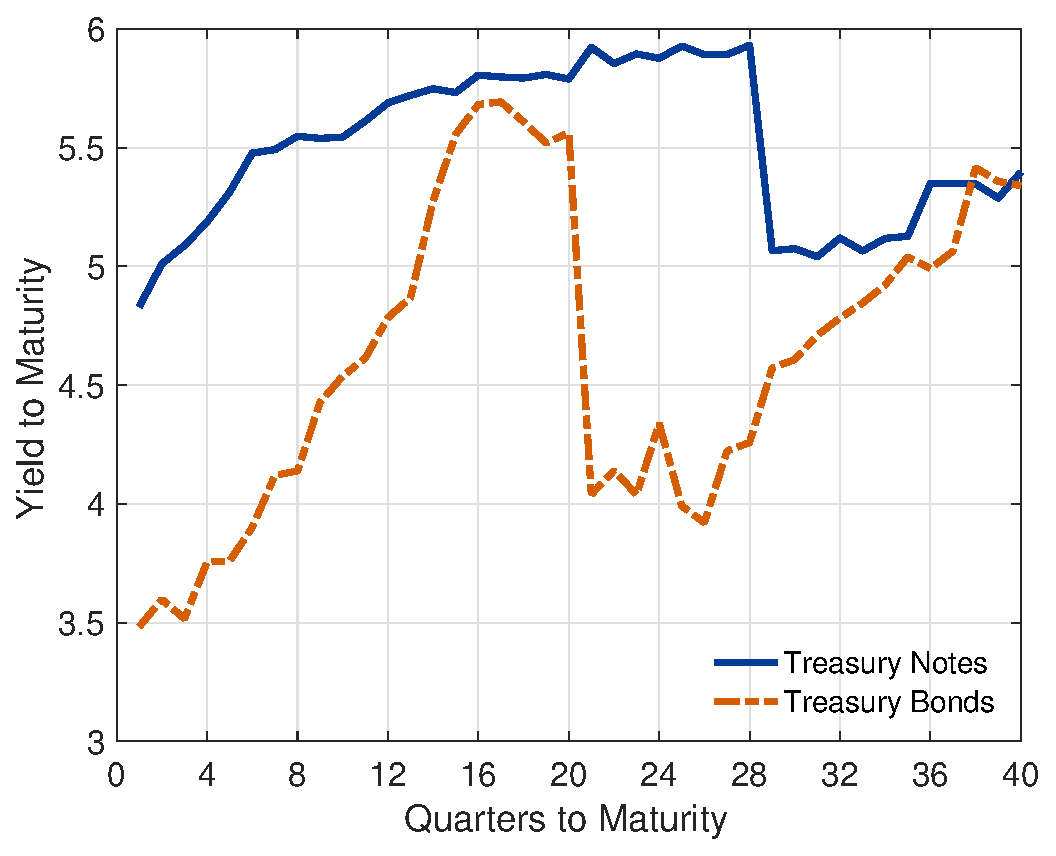
\includegraphics[width=0.7\textwidth]{../Figures/BondNote_Spread.eps}
% \caption{Median Treasury Bond and Note Yields with Same Time to Maturity}{(1970-2020)}
% \label{fig:YTM_Spread}
% \end{figure}
%: Median YTM Time Series
% \begin{figure}[p]
% \centering
% 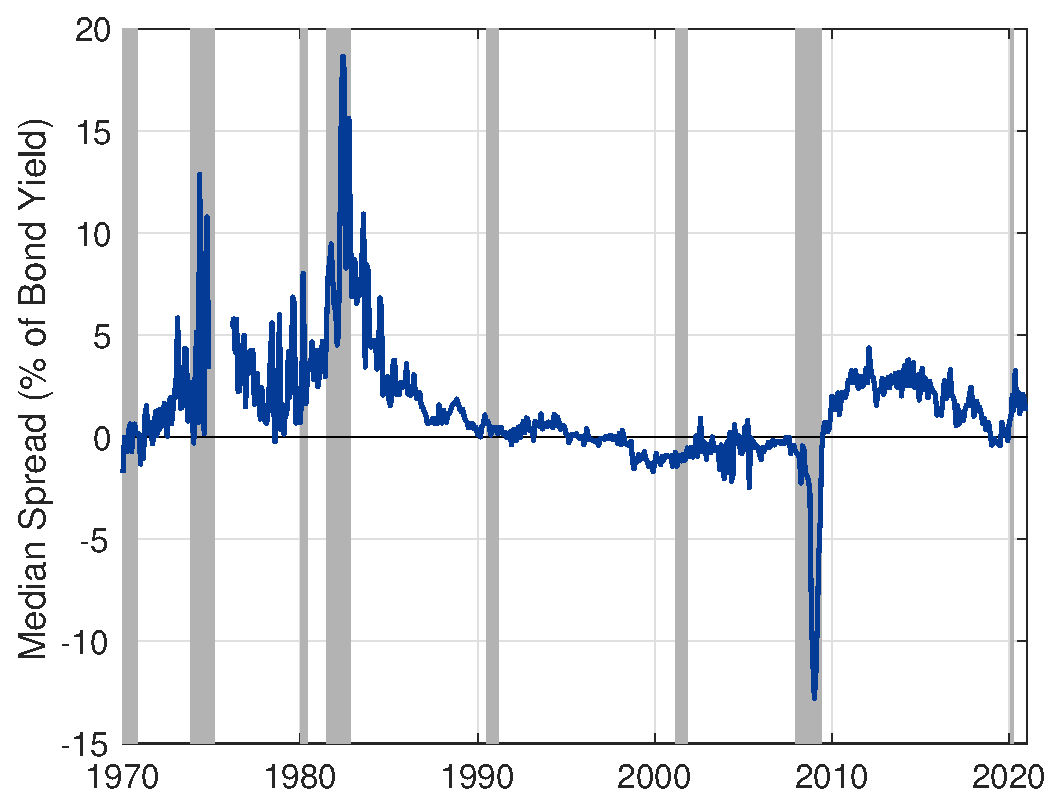
\includegraphics[width=0.7\textwidth]{../Figures/BondNote_TimeSeries.eps}
% \caption{Median Treasury Note--Bond Yield Spread with Same Time to Maturity}{(1970-2020)}
% \label{fig:YTM_SpreadTS}
% \end{figure}
%: Median Bid-Ask Spread over the Sample Period 
% \begin{figure}[h]
% \centering
% 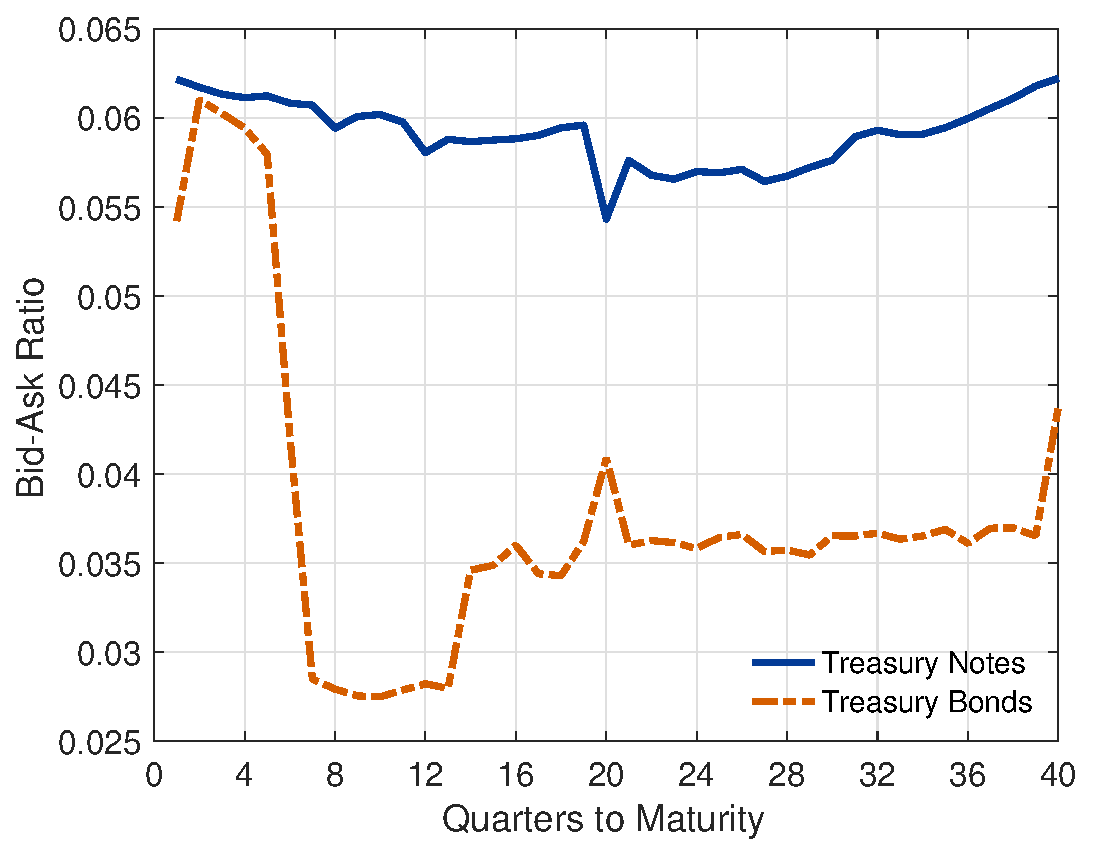
\includegraphics[width=0.7\textwidth]{../Figures/BidAsk_Ratios.eps}
% \caption{Median Treasury Bond and Note Bid-Ask Ratios with Same Time to Maturity}{(1970-2020)}
% \label{fig:BidAsk_Ratios}
% \end{figure}


\subsection{Hurdles in the Application}
\label{subsec:Hurdles}
One drawback of the T\"{o}rnqvist-Theil Divisia index is that it does not handle assets coming into and out of the market ($x_{j,t} = 0$ for some $t$) very well.
When calculating general monetary aggregates, this problem does not arise very often and is managed by imputing a reservation price and switching to a Fisher ideal index for those time periods.
Given the frequent changes in Treasury policy and the categorization I use, zero values are commonplace in this analysis.

To better account for zero values, I utilize the Fisher ideal index for the full sample.
This index still utilizes the user cost approach discussed above and is shown to be a Diewert-superlative index number like the Divisia index \citep{Diewert:1976}; but happens to be more applicable to the constraints of this particular dataset.
The Fisher ideal index (in levels) is expressed as
	\begin{equation}
		M^f_t = M^f_{t-1}\left[\frac{(\boldsymbol \eta_t \mathbf{m'}_t) (\boldsymbol \eta_{t-1} \mathbf{m'}_t)}{(\boldsymbol \eta_t \mathbf{m'}_{t-1}) (\boldsymbol \eta_{t-1} \mathbf{m'}_{t-1})}\right]^{\frac{1}{2}},
		\label{eq:FisherIdeal}
	\end{equation}
where $M^f_t$ denotes the new aggregate and the rest of the notation is defined above.
Since there is no initial value of this index $M^f_0$, the aggregate is first calculated in growth rates and then converted to a quantity index. 

\section{Theory}
\label{sec:Theory}
As \citet{Barnett:1980} outlines, aggregation theory relies on known, exact functional forms with estimable parameters.
The functions of interest are typically utility and production functions, which are often impossible to know.
This is why I rely on statistical index numbers, whose theory only relies on the existence of maximizing behavior.
From this optimizing behavior we can derive the user costs of the underlying components and bypass the unknown parameters because the resulting index numbers are not dependent on any specialized properties of the aggregator function.
That is, while I'm not deriving the true aggregate itself, the resulting quantity index will track the true aggregate.
A complete guide to index number theory and its application to monetary aggregation can be found in \citet{Barnett-Serletis:2000}.

A proper quantity index requires a price that is derived from an optimizing agent.
Thus, motivating the measurement of marketable government debt requires a partial equilibrium model that derives both the period-by-period user cost of holding government debt as well as the budgetary constraints the fiscal authority encounters.
This model incorporates both short- and long-term debt issued by the government, as well as an alternative long-term asset that will act as the benchmark asset. 
In this model, I refer to the alternative asset as ``capital,'' though it could also be motivated in some other fashion. 

\subsection{Long-Term Asset Dynamics}
The long-term government bonds and capital both evolve in a similar fashion.
As described by \citet{Krause-Moyen:2016}, each period new nominal long-term government bonds $B^{L,n}_t$ are issued, which are added to the stock of outstanding long-term debt $B^L_t$.
A portion $\alpha \in (0,1)$ of the previous period's stock of long-term bonds mature, while the remaining $(1-\alpha)$ remain in the stock of outstanding long-term debt. 
The maturity of these bonds is therefore $\sfrac{1}{\alpha}$.
Together, the stock of outstanding long-term debt evolves such that 
\begin{equation}
	B^L_t = (1-\alpha)B^L_{t-1} + B^{L,n}_t.
	\label{eq:LoM_DebtLevel}
\end{equation}
The average nominal interest rate paid on the stock of outstanding long-term debt $r^L_t$ evolves such that
\begin{equation}
	r^L_t B^L_t = (1-\alpha)r^L_{t-1}B^L_{t-1} + r^{L,n}_tB^{L,n}_t,
	\label{eq:LoM_DebtReturn}
\end{equation}
where $r^{L,n}_t$ is the interest rate on newly-issued long-term bonds. 

Capital is structured in a similar fashion, with the total stock of outstanding capital evolving according to
\begin{equation}
	K_t = (1-\delta)K_{t-1} + I_t,
	\label{eq:LoM_CapLevel}
\end{equation}
where $I_t$ is new investment in capital and $\delta \in (0,1)$ designates the portion of the outstanding stock of capital that matures each period.
This implies that the maturity of capital is $\sfrac{1}{\delta}$. 
The average interest rate paid on the capital stock outstanding $R_t$ is derived by
\begin{equation}
	R_tK_t = (1-\delta)R_{t-1}K_{t-1} + R^n_tI_t,
	\label{eq:LoM_CapReturn}
\end{equation}
where $R^n_t$ is the interest rate on newly-issued capital.

\subsection{Representative Household}
The representative household in this model works $l_t$ hours each period for nominal wage $W_t$, less an income tax rate $\tau_t$.
It also earns income through it's previous investments in capital $(\delta + R_{t-1})K_{t-1}$, short-term (one-period) bonds $(1+r_t)B_{t-1}$, long-term bonds $(\alpha + r^L_{t-1})B^L_{t-1}$, and profits from a continuum of intermediate goods-producing firms $\int^1_0 \Pi_t(s) \mathrm{d}s$.\footnote{
	The $\delta$ considered here can deviate from that in (\ref{eq:LoM_CapLevel}) if depreciation is considered.
	In this present study, however, we assume zero deprecation and treat ``capital'' as an alternative long-term security similar to the long-term government bond.
	Additionally, the inclusion/exclusion of the corporate profit term does not alter the results of this partial equilibrium setup, but would be needed in a full, general equilibrium presentation.}
This income is spread between a real consumption good $c_t$ at price $p_t$ as well as new investments in nominal short-term bonds $B_t$, long-term bonds $B^{L,n}_t$, and capital $I_t$.
Combined, the household's period-by-period budget constraint can be expressed as
\begin{multline}
	B_t + B^{L,n}_t + p_tc_t + I_t = (\delta + R_{t-1})K_{t-1} + (1+r_{t-1})B_{t-1} + \\ (\alpha + r^L_{t-1})B^L_{t-1} + (1-\tau_t)W_tl_t + \int^1_0\Pi_t(s)\text{d}s.
	\label{eq:HH_Budget}
\end{multline}

The household objective is to maximize utility over the real consumption good, the real monetary services provided by its portfolio of government bonds, and leisure
\begin{equation}
	\max\mathbb{E}_t\! \sum^\infty_{t=0} \beta^t\left\{u(c_t) + v\left(\frac{M_t}{P_t}\right) + x(1-l_t)\right\},
	\label{eq:HH_Utility}
\end{equation}
where $u(\cdot)$, $v(\cdot)$, and $x(\cdot)$ are increasing, concave functions. 
The monetary services provided by the portfolio are captured by a constant elasticity of substitution function 
\begin{equation}
	M_t = \left[\lambda^{\frac{1}{\sigma}}B_t^{\frac{\sigma-1}{\sigma}} + (1-\lambda)^{\frac{1}{\sigma}}{B^L_t}^{\frac{\sigma-1}{\sigma}}\right]^{\frac{\sigma}{\sigma-1}},
	\label{eq:HH_MonServices}
\end{equation}
where $\lambda \in [0,1]$ dictates the weight of each government debt security and $\sigma$ dictates the elasticity of substitution between the two assets.

Solving the household's problem results in the following dynamic conditions:
\begin{equation}
	1 - \gamma_{2,t}\left(\frac{\lambda M_t}{B_t}\right)^\frac{1}{\sigma} = \beta \mathbb{E}_t\!\left[\frac{\mu_{1,t+1}}{\mu_{1,t}}\frac{1+r_t}{\pi_{t+1}}\right],
	\label{eq:HH_manOC_B}
\end{equation}
%
\begin{multline}
	1 - \gamma_{2,t}\left(\frac{(1-\lambda)M_t}{B^L_t}\right)^\frac{1}{\sigma} + \gamma_{4,t}\left(r^L_t-r^{L,n}_t\right) \\
	= \beta \mathbb{E}_t\!\left[\frac{\mu_{1,t+1}}{\mu_{1,t}}\frac{1}{\pi_{t+1}} \left\{ 1+r^L_t + (1-\alpha)\gamma_{4,t+1} \left(r^L_t-r^{L,n}_{t+1}\right)\right\}\right],
	\label{eq:HH_manOC_BL}
\end{multline}
%
and
\begin{equation}
	1 + \gamma_{3,t}\left(R_t - R^{n}_t\right)  = \beta\mathbb{E}_t\!\left[\frac{\mu_{1,t+1}}{\mu_{1,t}}\frac{1}{\pi_{t+1}}\left\{ 1 + R_{t} + (1-\delta)\gamma_{3,{t+1}}\left(R_{t} - R^{n}_{t+1}\right)\right\}\right],
	\label{eq:HH_manOC_K}
\end{equation}
The solution technique to the household's problem can be found in Appendix \ref{app:HH_Solution}.
Here, $\mu_{1,t} = u'(c_t)$, $\gamma_{2,t} = \sfrac{v'(\cdot)}{u'(\cdot)}$, and $\gamma_{3,t}$ and $\gamma_{4,t}$ are the prices of the long-term assets $B^L_t$ and $K_t$, respectively.
These prices evolve according to
\begin{equation}
	\gamma_{3,t} = \beta\mathbb{E}_t\!\left[\frac{\mu_{1,t+1}}{\mu_{1,t}}\frac{1}{\pi_{t+1}} \left\{1 + (1-\delta)\gamma_{3,{t+1}}\right\}\right],
	\label{eq:HH_manOC_R}
\end{equation}
%
and
\begin{equation}
	\gamma_{4,t} = \beta\mathbb{E}_t\!\left[\frac{\mu_{1,t+1}}{\mu_{1,t}}\frac{1}{\pi_{t+1}} \left\{1 + (1-\alpha)\gamma_{4,{t+1}}\right\}\right].
	\label{eq:HH_manOC_rL}
\end{equation}

The user costs of the short- and long-term bonds are 
\begin{equation}
	\eta_t = \frac{\mathbb{E}_t \Big[ \frac{\mu_{t+1}}{\mu_{t}}\frac{1}{\pi_{t+1}} \Big\{ R^n_t - (1-\delta)\gamma_{3,t+1}\Delta R^n_{t+1} - r_t \Big\}\Big]}{\mathbb{E}_t \Big[ \frac{\mu_{t+1}}{\mu_{t}}\frac{1}{\pi_{t+1}} \Big\{ 1+ R^n_t - (1-\delta)\gamma_{3,t+1}\Delta R^n_{t+1}\Big\}\Big]},
\end{equation}
and
\begin{equation}
\eta^L_t = \frac{\mathbb{E}_t \Big[ \frac{\mu_{t+1}}{\mu_{t}}\frac{1}{\pi_{t+1}} \Big\{ R^n_t  - (1-\delta)\gamma_{3,t+1}\Delta R^n_{t+1} - r^{L,n}_t + (1-\alpha)\gamma_{4,t+1}\Delta r^{L,n}_{t+1}\Big\}\Big]}{\mathbb{E}_t \Big[ \frac{\mu_{t+1}}{\mu_{t}}\frac{1}{\pi_{t+1}} \Big\{ 1+ R^n_t - (1-\delta)\gamma_{3,t+1}\Delta R^n_{t+1}\Big\}\Big]},
\label{eq:usercost_LT}
\end{equation}
respectively.
The derivations of these user costs can be found in Appendix \ref{app:usercost_derivation}.

\subsection{Fiscal Capacity Considerations}
\label{subsec:Theory_Capacity}
\citet*{Brunnermeier-Merkel-Sannikov:2022} have shown that government debt constraints need to be augmented for the service flows (transaction/monetary services) that the securities provide.
Here I expand upon this idea with the specifics of the model above, providing a deeper look at how we can ascertain those services flows in particular.\footnote{
	This is identical to the exercise conducted by \citet{Brunnermeier-Merkel-Sannikov:2020}, though I abstract from the bubble term to focus solely on the monetary services component.}
Consider the simple budget constraint of the government in this model
\begin{equation}
	(1+r_{t-1})\frac{B_{t-1}}{p_t} + (\alpha + r^L_{t-1})\frac{B^L_{t-1}}{p_t} = \frac{B_t}{p_t} + \frac{B^{L,n}_t}{p_t} + s_t,
\end{equation}
where $s_t$ is denotes the real primary surplus. 
Now incorporate (\ref{eq:LoM_DebtLevel}) into the above equation to get
\begin{equation}
	(1+r_{t-1})\frac{B_{t-1}}{p_t} + (1 + r^L_{t-1})\frac{B^L_{t-1}}{p_t} = \frac{B_t}{p_t} + \frac{B^{L}_t}{p_t} + s_t.
\end{equation}
Since (\ref{eq:HH_manOC_B}) and (\ref{eq:HH_manOC_BL}) must hold,
\begin{multline}
	\frac{B_{t-1} + B^L_{t-1}}{p_t}(1+r_{t-1})= s_t  - (r_{t-1}^L - r_{t-1})\frac{B^L_{t-1}}{p_t} + \beta\mathbb{E}_t\left[\frac{\mu_{1,t+1}}{\mu_{1,t}} \frac{B_{t} +B^L_{t}}{p_{t+1}}(1+r_{t})\right] \\ 
		- \beta\mathbb{E}_t\left[\frac{\mu_{1,t+1}}{\mu_{1,t}} \frac{B^L_{t}}{p_{t+1}}(1+r_{t})\right] + \beta\mathbb{E}_t\left[\frac{\mu_{1,t+1}}{\mu_{1,t}} \frac{B^L_{t}}{p_{t+1}}(1+r^L_{t})\right] \\
		+  \gamma_{2,t}\left(\frac{\lambda M_t}{B_t}\right)^\frac{1}{\sigma}\frac{B_t}{p_t} +\gamma_{2,t}\left(\frac{(1-\lambda) M_t}{B^L_t}\right)^\frac{1}{\sigma}\frac{B^L_t}{p_t} \\
		+\beta\mathbb{E}_t\left[\frac{\mu_{1,t+1}}{\mu_{1,t}} \frac{B^L_t}{p_{t+1}}\left\{1+  (1-\alpha)\gamma_{4,t+1}\left(r^L_t - r^{L,n}_{t+1}\right)\right\}\right] - \gamma_{4,t}\left(r^L_t - r^{L,n}_t\right)\frac{B^L_t}{p_t}
\end{multline}
Including (\ref{eq:HH_manOC_rL}) and some rearranging, we can simplify the above equation to
\begin{multline}
	\frac{B_{t-1} + B^L_{t-1}}{p_t}(1+r_{t-1})= s_t - (r_{t-1}^L - r_{t-1})\frac{B^L_{t-1}}{p_t} + \beta\mathbb{E}_t\left[\frac{\mu_{1,t+1}}{\mu_{1,t}} \frac{B_{t} +B^L_{t}}{p_{t+1}}(1+r_{t})\right] \\ 
		+ \beta\mathbb{E}_t\left[\frac{\mu_{1,t+1}}{\mu_{1,t}} \frac{B^L_{t}}{p_{t+1}}(1+r^L_{t} - (1-\alpha)\gamma_{4,t+1}\Delta r^{L,n}_{t+1} - r_t)\right]  \\
		+  \gamma_{2,t}\left(\frac{\lambda M_t}{B_t}\right)^\frac{1}{\sigma}\frac{B_t}{p_t} +\gamma_{2,t}\left(\frac{(1-\lambda) M_t}{B^L_t}\right)^\frac{1}{\sigma}\frac{B^L_t}{p_t}.
\end{multline}

The last two terms are of particular importance here.
Incorporating the definition of the monetary services aggregate reduces the above expression to 
\begin{multline}
	\frac{B_{t-1} + B^L_{t-1}}{p_t}(1+r_{t-1})= s_t  - (r_{t-1}^L - r_{t-1})\frac{B^L_{t-1}}{p_t} + \beta\mathbb{E}_t\left[\frac{\mu_{1,t+1}}{\mu_{1,t}} \frac{B_{t} +B^L_{t}}{p_{t+1}}(1+r_{t})\right] \\ 
		+ \beta\mathbb{E}_t\left[\frac{\mu_{1,t+1}}{\mu_{1,t}} \frac{B^L_{t}}{p_{t+1}}(1+r^L_{t} - (1-\alpha)\gamma_{4,t+1}\Delta r^{L,n}_{t+1} - r_t)\right] 
		+  \gamma_{2,t}\frac{M_t}{p_t},
	\label{eq:fiscalcapacity}
\end{multline}
where it can be shown that
\begin{equation}
	\gamma_{2,t} = \left[\lambda \eta_t^{\sigma-1} + (1-\lambda)\left(\eta^L_t\right)^{\sigma-1}\right]^\frac{1}{\sigma-1}
	\label{eq:price_dual}
\end{equation}
is the price dual for the monetary services aggregate. 

There are a couple of items to point out with regards to the above expression.
First, fiscal capacity intuitively diminishes as long-term rates rise relative to short-term rates.
This term is reflecting the convenience yields that the government enjoys on its short-term debt.
Second, the fourth term on the right side suggests long-term debt can improve fiscal capacity via its longer maturity and a higher expected one-period return over the short-term debt. 
That is, while capacity shrinks with higher long-term interest rates, demand for the debt increases with higher expected holding-period returns. 
Lastly, fiscal capacity increases with the value of the monetary/transaction services the debt provides.
Thus, the monetary services provided by government debt issuances is directly captured in the government's budget constraint in a similar fashion to that shown in \citet{Brunnermeier-Merkel-Sannikov:2022}.


\section{Data and Methodology}
\label{sec:DataMethodology}
In this section, I construct the Fisher ideal quantity index described in Section \ref{sec:Theory} from data compiled by the Center for Research in Securities Prices on marketable Treasury securities.
Non-marketable debt is typically held by intergovernmental agencies, and is therefore not typically considered to be a significant burden.\footnote{
	The inclusion of only publicly-held, marketable US Treasury debt would be the optimal choice here, but data restrictions keep me from assessing this.
	For instance, the CRSP data doesn't include the amount of each T-bill issuance held publicly.
	Another option could be to exclude the issuances held by the Federal Reserve, since that is the primary non-public holder of US Treasuries, but the SOMA data only goes back to 2003.
	Future research could apply this methodology to the shortened timeframe.}
The Treasury began its ``regular and predictable'' debt issuance campaign in the 1970s and data regarding the spot and forward interest rates goes back to January 1977.
Therefore the variables constructed here will cover the February 1977 to December 2020 period.

The first issue that needs to be addressed is essentially analogous to new-product bias.
As (\ref{eq:FisherIdeal}) shows, the calculation of the growth rates requires both current and lagged quantities and user costs. 
If I were to treat each issuance as a separate $m_{i,t}$, there would be distortions at issuance and maturity months.
For example, in the issuance month of $m_{i,t}$, the preceding month's yield $r_{i,t-1}$ of that particular issuance doesn't exist, which means its user cost $\eta_{i,t-1}$ also doesn't exist.
Therefore, an assumption would need to be made regarding this lagged user cost.
\citet{Feenstra:1994} and others have outlined a theoretically justified solution to this problem in which the price is set at its reservation level, where the quantity demanded would equal zero in the preceding month.\footnote{
	The Center for Financial Stability, which publishes data on Divisia monetary aggregates, delays the inclusion of new monetary assets for a few months.
	In this situation, however, the regular issuance and maturity of short-term debt make this strategy problematic.}
It's also well documented that on-the-run bonds sell at a premium over their off-the-run counterparts, suggesting $\eta_{i,t-1} > \eta_{i,t}$, but by how much?
Estimating the reservation price of each issuance in each month over the sample period would seem to be too technically burdensome. 
With how distortionary this bias can be, some adjustments and/or assumptions are needed.

To reduce the magnitude of this issue, I cluster the assets into groups that are most likely to be perfect substitutes in any given month.
While there may be discrepancies in on-the-run/off-the-run securities, they should average out within the clusters. 
Based on the work of \citet{Amihud-Mendelson:1991} as well as the descriptive statistics in Figures \ref{fig:YTM_Spread} and \ref{fig:BidAsk_Ratios}, the securities need to be separated across their designation of {\em bills}, {\em notes}, and {\em bonds}.
Since 1997, the Treasury has issued Treasury Inflation-Protected Securities (TIPS), which yield a real rate of interest instead of the traditional nominal yield.
These have been shown to be less liquid than their nominal counterparts, so I create two additional categories of {\em TIPS notes} and {\em TIPS bonds}. 
Lastly, as these securities mature, their yields tend to fall with the trend of the constant maturity yield curve, reflecting the changing monetary services they provide.
Therefore, each of these five categories needs to be further segmented by their time to maturity.
Since bonds and longer notes are issued on a quarterly basis, it's common to have individual months where there are no securities of a certain type.\footnote{
	These notes and bonds are typically subject to reopenings in the months following the initial issuance, but the maturity dates are unchanged.
	For example, if a 30-year bond is issued in February, a reopening of that issuance may be offered in March, but the time-to-maturity on that reopening is 29 years, 11 months.}
A fine-grained segmentation such as this would again be subject to a large amount of new-product bias, so I define each sub-category as the quarters-to-maturity.
That is, for securities that will mature over the next one-to-three months, they are categorized has maturing within one quarter. 
A thirty-year threshold on bonds suggests 120 quarters-worth of categories, but there were a series of longer-term bonds that were issued between 1953 and 1965, which could impact the first years of the analysis.
Therefore, the number of quarters-to-maturity categories is set at 160, or forty years. 
Overall, when accounting for both the types of securities and the quarters to maturity, there are 800 categories.\footnote{
	Note that, based on (\ref{eq:FisherIdeal}), baskets that are consistently empty do not impact the measurement, allowing me to keep it consistent across the types of securities.
	So while there are 800 total baskets, a large number of them will not contribute to the measurement, but it does provide the flexibility needed for the aggregate over the almost fifty-year analysis.}
	
The next step in this process is to identify the proper interest rates from the theory above.
Since the user costs represent the holding period return and incorporate the interest rates paid on newly-issued securities ($r_t$ and $r^{L,n}_t$) and not on the average interest rate paid out on outstanding debt ($r^L_t$), the most accurate interest rates to consider are the coupon rates.
Additionally, the term $(1-\alpha)\gamma_{4,t+1}\Delta r^{L,n}_{t+1}$ represents the expected capital gains of the long-term bond. 
To account for these expectations, I use the current price of the bonds adjusted for its maturity, multiplied by the difference between the one-month-ahead forward rate and spot rate for each bond's particular month and maturity.
For TIPS, I consider the real spot and forward yield curves in the calculation of expected capital gains. 
While forward rates incorporate more than just future expectations of current spot rates, the impact of any term premium looking only one month ahead should be negligible.

The rate considered for each basket of securities is the quantity-weighted average over the issuances therein, though a further assumption is needed to address missing values/new-product bias.
As discussed above, even the broader categories used here do not ensure that there are no issues with new-product bias.
Since most of the empty categories in this situation are simply a cluster of maturing debt through time, and not new issuances of debt, I use the linear interpolation of the rates across the maturities instead of calculating a reservation rate.
This ensures that I'm capturing the true shape of the yield curves used. 

The benchmark rate used here is the maximum holding-period return of the baskets of securities considered each month, plus twenty-five basis points.\footnote{
	Previous iterations of this measurement attempted to use the Baa Corporate Bond yield, which would have accounted for both the liquidity and safety attributes of Treasury securities.
	However, even the addition of 200 basis points did not ensure that all user costs were positive across the sample period, especially in the volatile years of 1979--1981 and long periods of time between 2014 and 2016.
	Adjustments to create that kind of spread for the early years also had the drawback of washing out the differences in user costs in the later parts of the sample period.}
This is similar to the strategy used by the Federal Reserve in their calculation of Divisia monetary aggregates and is common in other derivations of user costs. 

\section{Results}
\label{sec:Results}

\subsection{The Measure}
\label{subsec:Results_Measure}

The month-over-month growth rates of both the true aggregate and its simple sum counterpart are constructed from the data.
This indirect approach to the aggregates' levels is necessary as there is no initial value from which to begin the calculation of (\ref{eq:FisherIdeal}).
Simply taking the logarithm of (\ref{eq:FisherIdeal}) yields the growth-rate variation used.
The general levels of the growth rates are similar, so I present their spread in Figure \ref{fig:Growth_Spread}.
To aid in the visual analysis, the 12-month moving average (centered on the seventh month) spread of these growth rates is superimposed.
As can be seen, the true aggregate tends to grow faster than the simple sum aggregate, but there are also periods of relatively slow growth.
%: Differences in the Aggregates' Growth Rates
% \begin{figure}[h]
% \centering
% 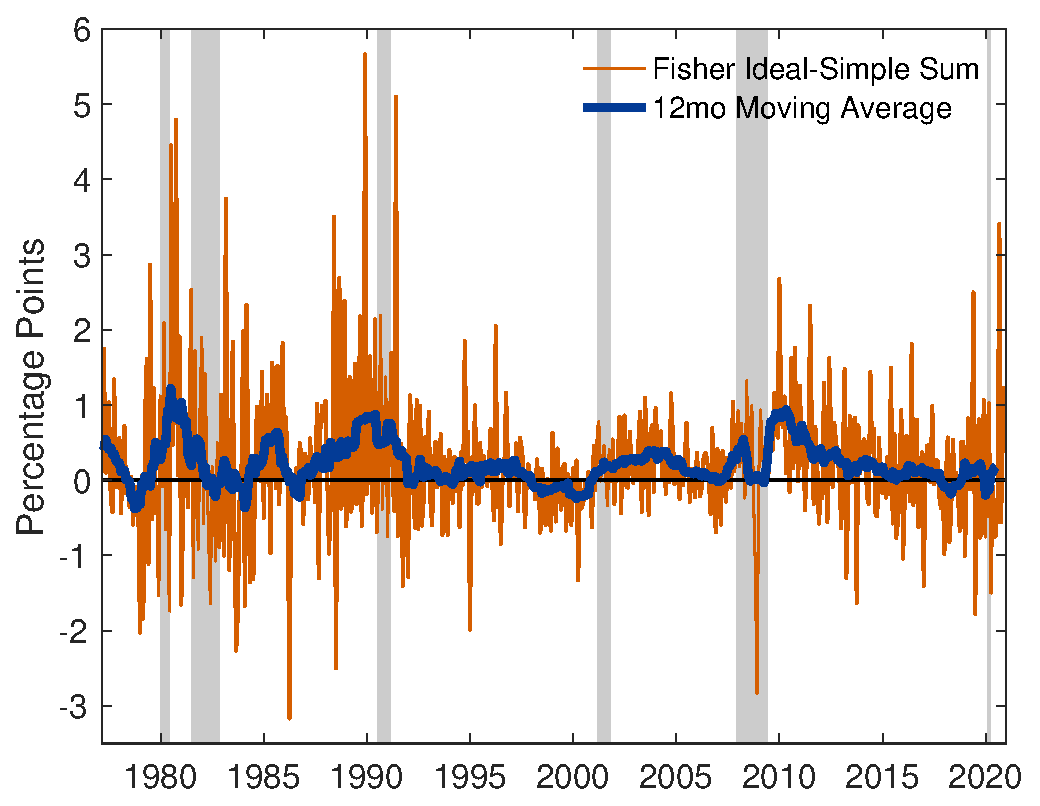
\includegraphics[width=0.85\textwidth]{../Figures/GrowthDiff_v2.eps}
% \caption{Month-over-month Growth Rate Spread}
% \label{fig:Growth_Spread}
% \end{figure}

Since the true aggregate incorporates both the quantities of the underlying assets and the monetary services they provide, the spread intuitively reveals the growth of these monetary services alone.
That is, I am essentially factoring-out the growth that comes purely from the issued principal values.
The spread in Figure \ref{fig:Growth_Spread}, therefore, represents the growth of fiscally-provided monetary services.
This figure shows us that the Treasury generally adds to the stock of monetary services over time, with notable exceptions in the late-1990s when the government was running a fiscal surplus.
In that instance, the growth rates suggest that the monetary services provided were shrinking along with the principal values. 


%: Index Values of the Monetary Services
% \begin{figure}[h]
% \centering
% \includegraphics[width=0.85\textwidth]{../Figures/MonetaryServices_Index.eps}
% \caption{Monetary Services Level}
% \label{fig:MS_Index}
% \end{figure}
Using these growth rate spreads, I derive an index that tracks the stock of monetary services, shown in Figure \ref{fig:MS_Index}.
Multiple theories have claimed that Treasury securities provide services above and beyond their principal value, but this is the first attempt to measure such services. 
The base month considered here is August 1989 due to the relative flatness of the yield curve at that time.
When the yield curve is flat, the differences in the user costs are minimal, suggesting that the underlying assets are perceived as near-perfect substitutes and collapsing the Fisher ideal index into a simple sum aggregate.


\newpage

\bibliographystyle{apecon}
\bibliography{MonetaryServices_Debt}


\end{document}